\documentclass{tudphygp_eng}
\usepackage{xcolor,verbatim,moreverb,listings,wrapfig}
\usepackage[numbers]{natbib}
\lstset{basicstyle=\footnotesize\ttfamily}

\versuch{X-ray}{ROE}
\author{J.~Kr�mer}
\bearbeitet{engl. R.Mertzig}{}


\begin{document}

\maketitle

\section{Task}
Analyze either with a KBr- or with a LiF-crystal the characteristic x-rays of copper, iron, molybdenum and wolfram. Identify the atomic transitions, which create the measured lines in the x-ray spectrum, and calculate the corresponding energies.

\section{Theoretical basics}
Wilhelm Conrad R�ntgen discovered a new kind of ray through experiments with an electric discharge tube on November 8th, 1895. He named them X-rays. The X-rays are named after him in the German science community. 
R�ntgen proved that x-rays are created by electrons impacting on solids.
He was awarded for his discovery with the first Nobel prize in physics in 1901 \cite{NPR}.\\

Max von Laue proved some years later that x-rays are electromagnetic waves which are interfering with mono-crystals. He was awarded too with the Nobel prize in physics in the year 1914 \cite{NPL}. His method proving the uniformity of the structure of a crystal is still used today (Laue-diagrams). 
Father and son, William and Lawrence Bragg have to be mentioned as the third Nobel prize winners, who were awarded for investigations of crystal structures with x-rays in the following year 1915 \cite{NPB}.\\
X-rays are located in the partial intersection of the electromagnetic spectrum between UV and gamma rays at wavelengths in the range between 10\,nm and 1\,pm. 
X-rays have ionizing effects and can harm the human body and cause cancer. 
Therefore one has to obey radiative protection procedures while working with x-rays. The x-ray device is equipped with special protection glass and protective features for this experiment. 
The x-ray tube can be used only when the slide door is closed.\\
The x-ray is variously used for different applications nowadays, for instance for medical imaging or x-ray therapies, crystallography, microscopy and spectroscopy.
\begin{figure}[htbp]
\centering
\includegraphics[width=0.85\textwidth]{images/787px-EM_spectrum.png}
\caption{Electromagnetic spectrum, source: Wikipedia}
\label{fig:em-spektrum}
\end{figure}

\subsection{The x-ray tube}

A x-ray tube consists of two electrodes positioned in an evacuated glass tube. Electrons were created at the cathode through thermionic emission and were accelerated towards the anode. The acceleration potential between cathode and anode is defined as anode potential $U_{Anode}$ resp. $U_A$. Its typical range is usually between 10 and 100\,keV. In this experiment 35\,keV is applied. Electrons impacting on the anode release their energy partly as electromagnetic rays - the x-rays.
The bigger part will be transformed into heat.
\begin{figure}[htbp]
\centering
\includegraphics[width=0.7\textwidth]{images/roehre.png}
\caption{Setup of a x-ray tube.}
\label{fig:roehre}
\end{figure}


\subsection{The x-ray spectrum}
Two processes are important for creating x-rays at the anode. First, the electrons are scattered or decelerated in the Coulomb-field at the nuclei in the anode. They release energy of different amount as x-ray photons (x-rays) resulting in a continuous spectrum, named as "`Brems-spectrum"'. 
The energy of the brems radiation is limited by the energy conservation. The upper limit of the energy of the photons is the kinetic energy of the electron $e\cdot U_A$ gained by following the anode potential.
Usually the spectrum is plotted dependent to the wavelength $\lambda$ and not energy dependent.
 With the relation
\begin{align}
E=h\,f= \frac{h\,c}{\lambda}, \label{eq:E=}
\end{align}
and $h=6.626\cdot 10^{-34}$ Js (the Planck constant) and $c=2.998\cdot 10^8$ m/s (light speed in vacuum), the lower wavelength limit $\lambda_{min}$ in the brems spectrum can be derived:
\begin{align}
\lambda_{min}=\frac{h\,c}{e\,U_A}. \label{eq:planck}
\end{align}
\begin{figure}[htb]
\centering
\includegraphics[width=0.6\textwidth]{images/schema_spektrum.pdf}
\caption{A schematic figure of a x-ray spectrum.}
\label{fig:schema_spektrum}
\end{figure}
\\The continuous spectrum is superimposed by material characteristic lines. The electrons accelerating towards the anode have an ionizing effect. If they have enough kinetic energy they might ionize the strongly bounded electrons from the inner shells of the atoms of the anode. The vacancies can be re-occupied by electrons from the outer shells. The energy difference between both shells resp. energy levels can be released by photons. The difference of the energy levels equals the released photon energy.\\
As an example the energy levels for copper are shown in fig.~\ref{fig:energieniveaus}. 
The shells are named as  K-, L-, M-shells with the quantum numbers $n=1,2,3$ . $L$- and $M$-shells are 
further split into the fine structure determined by the angular momentum and quantum spin number.
Characteristic radiation generated by transitions from the $L$- to the $K$-shell are named $K_\alpha$-radiation, transitions from the $M$- to the $K$-shell are named $K_\beta$-radiation.
Rules for selection defined by the quantum-mechanical conservation laws forbid some transitions, for instance from $L_1$ to $K$ or $M_1$ to $K$.
The characteristic energy of the radiation can be determined from the energy level scheme, for instance for the $K_\beta$ radiation of copper: $8978.9\,\text{eV} - 73.6\,\text{eV} = 8.905\,\text{keV}$.\\
The energy level schemes for the other materials are listed in the appendix.
\begin{figure}[htbp]
\centering
\setlength{\fboxsep}{2.0mm}
\fbox{\includegraphics[width=0.6\textwidth]{images/scheme_Cu.png}}
\caption{The energy level scheme of copper, Source: PHYWE.}
\label{fig:energieniveaus}
\end{figure}

\subsection{Bragg-reflection}
\begin{wrapfigure}{r}{0.45\textwidth}
\centering
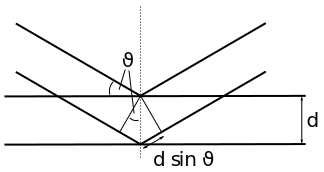
\includegraphics[width=0.4\textwidth]{images/braggdrawing.pdf}
\caption{Bragg-Reflection in the glancing angle $\vartheta$ at two lattice planes.}
\label{fig:bragg}
\end{wrapfigure}
X-rays intercepting the crystal at a certain angle will be reflected at the surface and at the lower lattice planes of that solid. Comparing two rays, which are reflected at the neighboring lattice planes, allow the deviation of the conditions for a constructive interference of those two rays. 
The phase difference $\Delta$ between both rays, as seen in the sketch, is dependent on the incident angle $\vartheta$ and the distance between two lattice planes $d$ . 

\begin{align}
\Delta = 2d\sin{\vartheta}
\end{align}
The reflected rays are in phase and constructively interfere if the phase difference is an integer of the wavelength.
In all other cases the huge number of lattice planes and reflections are causing the annihilation of the rays. The Bragg-equation is therefore:
\begin{align}
2d \sin{\vartheta}=n\,\lambda, \label{eq:Bragg}
\end{align}
with $d=$ the distance between the lattice planes and $n=$ the order of deflection. 
The reflected x-rays are monochromatized and the wavelength can be determined from the angle $\vartheta$, the glance angle, and from the distance between the lattice planes, $d$ . 
This effect is used with the "`rotating crystal method"' for analyzing the x-ray spectrum.\\
LiF or KBr, where the distance between the lattice planes is well known (see appendix), will be used as mono-crystal in this experiment. 
The energy of the radiation can be calculated with the Bragg-equation and eq.~\eqref{eq:E=}:
\begin{align}
E=\frac{n\,h\,c}{2d\,\sin{\vartheta}}. \label{eq:E_Xrays}
\end{align}


\subsection{Rotating crystal method}
\begin{figure}[htbp]
\centering
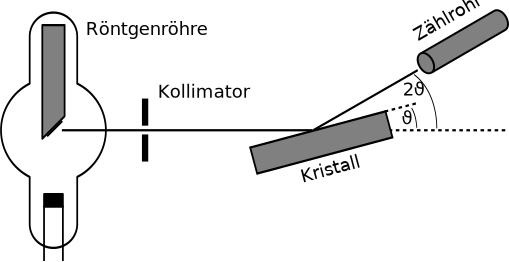
\includegraphics[width=0.6\textwidth]{images/drehkristall.pdf}
\caption{Measurement of an x-ray spectrum with the rotating crystal method}
\label{fig:drehkristall}
\end{figure}
X-rays impinge on a rotating crystal at the angle $\vartheta$ and are reflected. The resulting angle of the reflected radiation is always as twice as large as the angle of the crystal. The detector (the Geiger counter) has to be always in the position of a constant angular ratio for determining the x-ray spectrum with the rotating crystal method.\\

With this method one measures the intensity of the x-rays dependent on the angle of the crystal, which is named as the glance angle in the literature. From the plot of these measurements one can, for instance, determine the wavelengths of the characteristic lines from the Bragg-equation. The characteristic lines of the spectrum also appear in the spectrum as higher orders of diffraction ($n > 1$ s. eq.~\eqref{eq:Bragg}) . 
A spectrum of a copper anode measured at this setup is shown in Fig.~\ref{fig:spectrum_copper}.
\begin{figure}[htbp]
\centering
\includegraphics[width=0.9\textwidth]{images/spectrum_Cu_LiF.png}
\caption{Characteristic x-ray spectrum of copper as a function of the glance angle $\vartheta$ done with a LiF analysis crystal, Source: PHYWE.}
\label{fig:spectrum_copper}
\end{figure}


\section{Execution of the experiment}
\subsection{Setup and calibration}
A fully equipped setup can be used for this experiment (Fig.~\ref{fig:messplatz}). 
X-ray tubes with various anode materials, like wolfram, copper, iron and molybdenum are available. 
Insert the tube-containing frame into the x-ray device. Take the 2\,mm collimator aperture from the shelf of the x-ray device (lower down) and insert it as shown in Fig.~\ref{fig:Blende} .
 Choose either LiF or KBr as analyzing crystal and insert the crystal adjusting holder into the correct holes at the goniometer. The Geiger-M�ller counter, which is mounted at the end of the arm of the goniometer, will be used as the detector. The x-ray device can be controlled either with the control panel or connected via USB to a computer with the software \emph{measure} .\\ 

\begin{figure}[tbp]
\centering
\includegraphics[width=0.8\textwidth]{images/phywe_unit.jpg}
\caption{PHYWE X-ray expert unit.}
\label{fig:messplatz}
\end{figure}
\begin{figure}[tbp]
\centering
\includegraphics[width=0.8\textwidth]{images/aufbau.png}
\caption{Setup of the experimental area with the goniometer and the insertion of the collimator aperture, Source: PHYWE.}
\label{fig:Blende}
\end{figure}
The x-ray device can be turned on after inserting and connecting all components.
The goniometer has to be calibrated before starting the experiment. 
The choice of the analysis crystal has to fed in at the control panel of the x-ray device, then the auto calibration can be started (at Goniometer - Parameter - Kristall and then Goniometer - Autokalibrierung).  
The auto calibration and the following measurements can be started after the glass door is closed and locked (lock symbol at the device).

\subsection{Tasks}
Start the program \emph{measure}. 
You can change the corresponding settings by clicking on the different areas of the displayed x-ray device (Abb.~\ref{fig:measure}). 
Check the settings of the tube, if the tube potential is adjusted to 35\,kV and emission current is adjusted to 1\,mA. The settings of the goniometer have to be adjusted according to the choice of the x-ray tube and the analyzing crystal. One has to choose the angle of detection that the reflected x-rays can be measured in the glance angle. That means that the value of the angle of detection has to be always as twice as large as the angle of the crystal (compare Fig.~\ref{fig:bragg}) . This fixed ratio is automatically kept in the mode "`1:2 Kopplung"' . 
\begin{figure}[tbp]
\centering
\includegraphics[width=0.5\textwidth]{images/einstellungen.png}
\caption{Tube and goniometer settings with the program \emph{measure}, Source: PHYWE.}
\label{fig:measure}
\end{figure}
\begin{figure}[tbp]
\centering
\includegraphics[width=0.9\textwidth]{images/einstellungendialog.png}
\caption{Tube and goniometer settings, Source: PHYWE.}
\label{fig:einstellungen}
\end{figure}
\begin{table}[htbp]
\begin{center}
\begin{tabular}{|l||l|r|r|r|r|}
\hline
Anode material	& Crystal	& Starting angle		& Stopping angle	& Step size	& Integration time\\
\hline\hline
Cu				& LiF		& 4�				& 55�		& 0,1�		& 2\,s\\
\hline
Cu				& KBr	& 3�				& 75�		& 0,1�		& 2\,s\\
\hline
Fe				& LiF		& 4�				& 80�		& 0,1�		& 2\,s\\
\hline
Fe				& KBr	& 4�				& 65�		& 0,1�		& 2\,s\\
\hline
Mb				& LiF		& 3�				& 65�		& 0,1�		& 2\,s\\
\hline
Mb				& KBr	& 3�				& 30�		& 0,1�		& 2\,s\\
\hline
W				& LiF		& 4�				& 80�		& 0,1�		& 6\,s\\
\hline
\end{tabular}
\end{center}
\caption{Settings of the goniometer}
\label{tab:Goniometer}
\end{table}

\begin{center}
\setlength{\fboxsep}{4.0mm}
\fbox{\begin{minipage}{0.9\textwidth}
{\color{red}Caution}: Don't adjust to any angles smaller than 3� to avoid that the Geiger-M�ller-counter is exposed to the primary beam!
\end{minipage}}
\end{center}

\textbf{Hints for using the programm \emph{measure}:}\\
Click the \emph{record} button to start the experiment. Click "alle Messungen an measure �bertragen" after the measurement. First save your measurement and then evaluate the characteristic spectrum. For that you can use the features of \emph{measure}. Select the area of the spectrum where you want to analyze the peaks and click \emph{Peakanalyse}. Calculate the corresponding energy $E$ of the x-rays from the angles of the centers of the peaks considering their diffraction order. Calculate the corresponding measurement uncertainty $\Delta E$ of the energy from the characteristic width of the peaks.


\section{Questions}

\begin{enumerate}
	\item At which wavelengths and in which energy range are x-rays located?
	\item Which different x-ray spectra have to be distinguished?
	\item Why is there a short-wave limit in the brems spectrum?
	\item How is a characteristic x-ray spectrum created?
	\item What is the Bragg-equation?
	\item How does the rotating crystal method work?
\end{enumerate}

\nocite{*}
\bibliography{literature}
\bibliographystyle{unsrtdinat}



\clearpage

\section{Appendix}
%Energienieveauschemata
\begin{figure}[htbp]
\centering
\setlength{\fboxsep}{2.0mm}
\fbox{\includegraphics[width=0.6\textwidth]{images/scheme_Fe.png}}
\caption{Energy level scheme of iron, Source: PHYWE.}
\end{figure}
\begin{figure}[htbp]
\centering
\setlength{\fboxsep}{2.0mm}
\fbox{\includegraphics[width=0.6\textwidth]{images/scheme_Mb.png}}
\caption{Energy level scheme of molybdenum, Source: PHYWE.}
\end{figure}
\begin{figure}[htbp]
\centering
\setlength{\fboxsep}{2.0mm}
\fbox{\includegraphics[width=0.9\textwidth]{images/scheme_W.png}}
\caption{Energy level scheme of wolfram, Source: PHYWE.}
\end{figure}

\begin{table}[htbp]
	\begin{tabular}{lll}
		Planck-constant	& $h$	& $=6.6256\cdot 10^{-34}$ J\,s\\
		Speed of light	& $c$	& $=2.9979\cdot 10^{8}$ m/s\\
		distance of the lattice layers LiF (200)	& $d$	& $=2.014\cdot 10^{-10}$ m\\
		distance of the lattice layers KBr (200)	& $d$	& $=3.290\cdot 10^{-10}$ m\\
																& $1$ eV	& $=1.6021\cdot 10^{-19}$ J
	\end{tabular}
	\caption{Constants}
	\label{tab:Konstanten}
\end{table}
\end{document}
